\documentclass{standalone}
\usepackage{tikz}
\usetikzlibrary{patterns, positioning}


\begin{document}
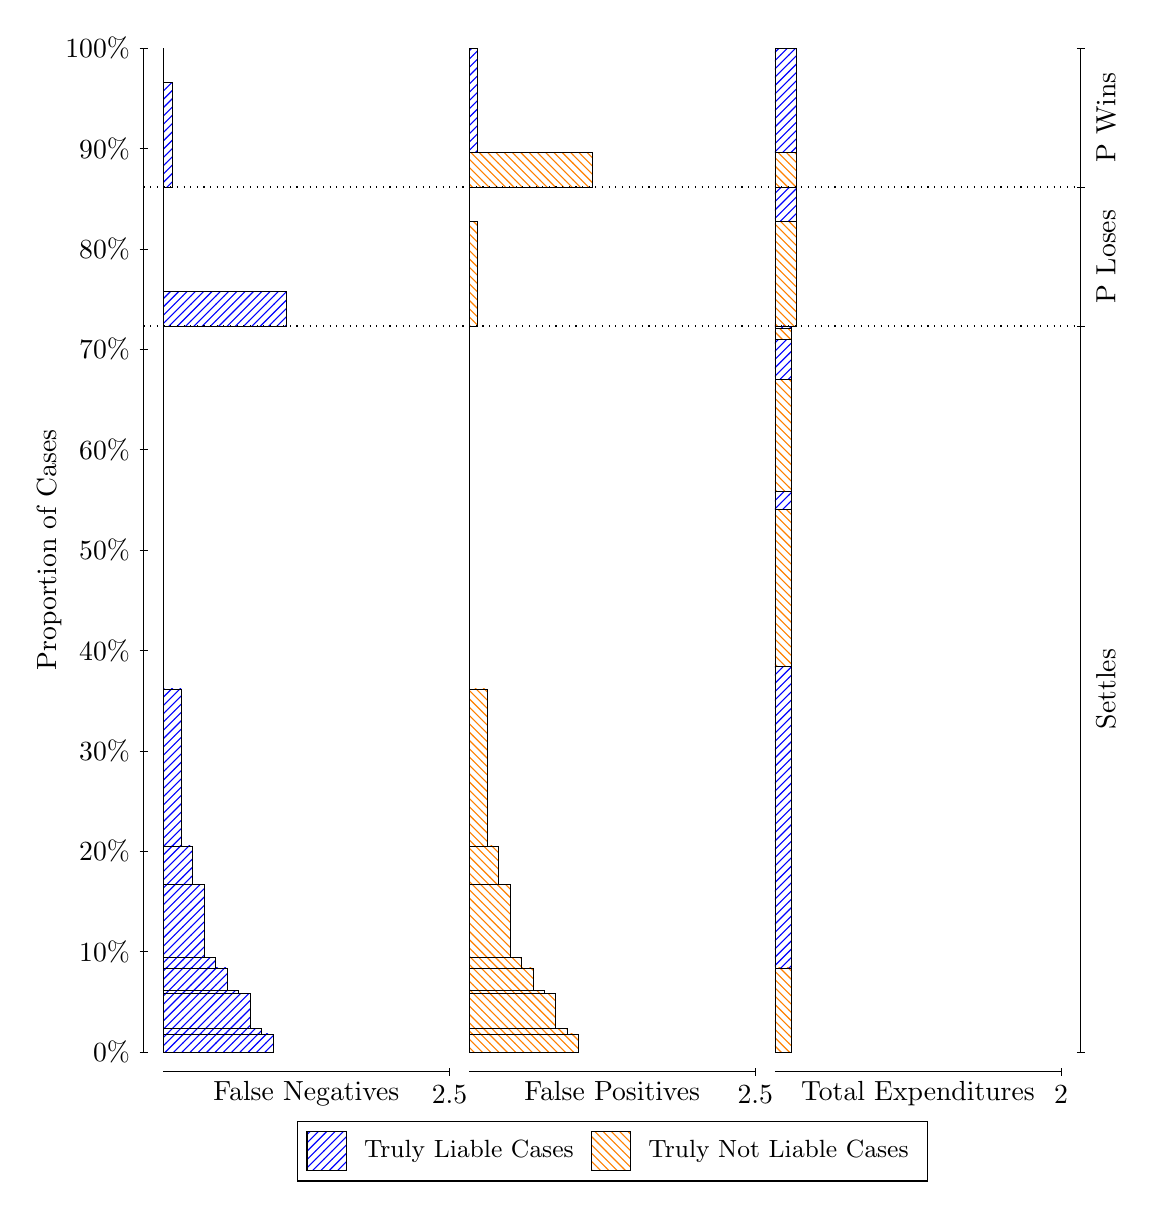
\begin{tikzpicture}
\draw[black, very thin] (1.5,1.75) -- (1.5,14.5);
\node[rotate=90, text=black, anchor=center] at (0.3, 8.125) {Proportion of Cases};
\draw[black, very thin] (1.45,1.75) -- (1.55,1.75);
\node[text=black, anchor=east] at (1.45, 1.75) {0\%};
\draw[black, very thin] (1.45,3.025) -- (1.55,3.025);
\node[text=black, anchor=east] at (1.45, 3.025) {10\%};
\draw[black, very thin] (1.45,4.3) -- (1.55,4.3);
\node[text=black, anchor=east] at (1.45, 4.3) {20\%};
\draw[black, very thin] (1.45,5.575) -- (1.55,5.575);
\node[text=black, anchor=east] at (1.45, 5.575) {30\%};
\draw[black, very thin] (1.45,6.85) -- (1.55,6.85);
\node[text=black, anchor=east] at (1.45, 6.85) {40\%};
\draw[black, very thin] (1.45,8.125) -- (1.55,8.125);
\node[text=black, anchor=east] at (1.45, 8.125) {50\%};
\draw[black, very thin] (1.45,9.4) -- (1.55,9.4);
\node[text=black, anchor=east] at (1.45, 9.4) {60\%};
\draw[black, very thin] (1.45,10.675) -- (1.55,10.675);
\node[text=black, anchor=east] at (1.45, 10.675) {70\%};
\draw[black, very thin] (1.45,11.95) -- (1.55,11.95);
\node[text=black, anchor=east] at (1.45, 11.95) {80\%};
\draw[black, very thin] (1.45,13.225) -- (1.55,13.225);
\node[text=black, anchor=east] at (1.45, 13.225) {90\%};
\draw[black, very thin] (1.45,14.5) -- (1.55,14.5);
\node[text=black, anchor=east] at (1.45, 14.5) {100\%};

\draw[black, very thin] (13.4,1.75) -- (13.4,14.5);
\draw[black, very thin] (13.35,1.75) -- (13.45,1.75);
\node[anchor=west] at (13.35, 1.75) {};
\draw[black, very thin] (13.35,10.97) -- (13.45,10.97);
\node[anchor=west] at (13.35, 10.97) {};
\draw[black, very thin] (13.35,12.735) -- (13.45,12.735);
\node[anchor=west] at (13.35, 12.735) {};
\draw[black, very thin] (13.35,14.5) -- (13.45,14.5);
\node[anchor=west] at (13.35, 14.5) {};

\draw[black, very thin, pattern color=blue, pattern=north east lines] (1.75,1.75) rectangle (3.1398,1.9792);
\draw[black, very thin, pattern color=blue, pattern=north east lines] (1.75,1.9792) rectangle (2.9944,2.0461);
\draw[black, very thin, pattern color=blue, pattern=north east lines] (1.75,2.0461) rectangle (2.8491,2.4941);
\draw[black, very thin, pattern color=blue, pattern=north east lines] (1.75,2.4941) rectangle (2.7037,2.5293);
\draw[black, very thin, pattern color=blue, pattern=north east lines] (1.75,2.5293) rectangle (2.5584,2.8167);
\draw[black, very thin, pattern color=blue, pattern=north east lines] (1.75,2.8167) rectangle (2.4131,2.9473);
\draw[black, very thin, pattern color=blue, pattern=north east lines] (1.75,2.9473) rectangle (2.2678,3.8763);
\draw[black, very thin, pattern color=blue, pattern=north east lines] (1.75,3.8763) rectangle (2.1224,4.3687);
\draw[black, very thin, pattern color=blue, pattern=north east lines] (1.75,4.3687) rectangle (1.9771,6.3601);
\draw[black, very thin, pattern color=orange, pattern=north west lines] (1.75,6.3601) rectangle (1.75,10.97);
\draw[black, very thin, pattern color=blue, pattern=north east lines] (1.75,10.97) rectangle (3.3123,11.406);
\draw[black, very thin, pattern color=orange, pattern=north west lines] (1.75,11.406) rectangle (1.75,12.735);
\draw[black, very thin, pattern color=blue, pattern=north east lines] (1.75,12.735) rectangle (1.859,14.064);
\draw[black, very thin, pattern color=orange, pattern=north west lines] (1.75,14.064) rectangle (1.75,14.5);
\draw[black, very thin, pattern color=orange, pattern=north west lines] (5.6333,1.75) rectangle (7.0231,1.9792);
\draw[black, very thin, pattern color=orange, pattern=north west lines] (5.6333,1.9792) rectangle (6.8777,2.0461);
\draw[black, very thin, pattern color=orange, pattern=north west lines] (5.6333,2.0461) rectangle (6.7324,2.494);
\draw[black, very thin, pattern color=orange, pattern=north west lines] (5.6333,2.494) rectangle (6.5871,2.5293);
\draw[black, very thin, pattern color=orange, pattern=north west lines] (5.6333,2.5293) rectangle (6.4417,2.8166);
\draw[black, very thin, pattern color=orange, pattern=north west lines] (5.6333,2.8166) rectangle (6.2964,2.9473);
\draw[black, very thin, pattern color=orange, pattern=north west lines] (5.6333,2.9473) rectangle (6.1511,3.8763);
\draw[black, very thin, pattern color=orange, pattern=north west lines] (5.6333,3.8763) rectangle (6.0057,4.3687);
\draw[black, very thin, pattern color=orange, pattern=north west lines] (5.6333,4.3687) rectangle (5.8604,6.3602);
\draw[black, very thin, pattern color=blue, pattern=north east lines] (5.6333,6.3602) rectangle (5.6333,10.97);
\draw[black, very thin, pattern color=orange, pattern=north west lines] (5.6333,10.97) rectangle (5.7423,12.3);
\draw[black, very thin, pattern color=blue, pattern=north east lines] (5.6333,12.3) rectangle (5.6333,12.735);
\draw[black, very thin, pattern color=orange, pattern=north west lines] (5.6333,12.735) rectangle (7.1957,13.171);
\draw[black, very thin, pattern color=blue, pattern=north east lines] (5.6333,13.171) rectangle (5.7423,14.5);
\draw[black, very thin, pattern color=orange, pattern=north west lines] (9.5167,1.75) rectangle (9.721,2.8166);
\draw[black, very thin, pattern color=blue, pattern=north east lines] (9.5167,2.8166) rectangle (9.721,6.6475);
\draw[black, very thin, pattern color=orange, pattern=north west lines] (9.5167,6.6475) rectangle (9.721,8.639);
\draw[black, very thin, pattern color=blue, pattern=north east lines] (9.5167,8.639) rectangle (9.721,8.8682);
\draw[black, very thin, pattern color=orange, pattern=north west lines] (9.5167,8.8682) rectangle (9.721,10.29);
\draw[black, very thin, pattern color=blue, pattern=north east lines] (9.5167,10.29) rectangle (9.721,10.804);
\draw[black, very thin, pattern color=orange, pattern=north west lines] (9.5167,10.804) rectangle (9.721,10.935);
\draw[black, very thin, pattern color=blue, pattern=north east lines] (9.5167,10.935) rectangle (9.721,10.97);
\draw[black, very thin, pattern color=orange, pattern=north west lines] (9.5167,10.97) rectangle (9.7892,12.3);
\draw[black, very thin, pattern color=blue, pattern=north east lines] (9.5167,12.3) rectangle (9.7892,12.735);
\draw[black, very thin, pattern color=orange, pattern=north west lines] (9.5167,12.735) rectangle (9.7892,13.171);
\draw[black, very thin, pattern color=blue, pattern=north east lines] (9.5167,13.171) rectangle (9.7892,14.5);
\draw[black, dotted] (1.5,10.97) -- (13.4,10.97);
\draw[black, dotted] (1.5,12.735) -- (13.4,12.735);
\draw[black, very thin] (1.75,1.5) -- (5.3833,1.5);
\node[text=black, anchor=north] at (3.5667, 1.5) {False Negatives};
\draw[black, very thin] (5.3833,1.45) -- (5.3833,1.55);
\node[text=black, anchor=north] at (5.3833, 1.45) {2.5};

\draw[black, very thin] (5.6333,1.5) -- (9.2667,1.5);
\node[text=black, anchor=north] at (7.45, 1.5) {False Positives};
\draw[black, very thin] (9.2667,1.45) -- (9.2667,1.55);
\node[text=black, anchor=north] at (9.2667, 1.45) {2.5};

\draw[black, very thin] (9.5167,1.5) -- (13.15,1.5);
\node[text=black, anchor=north] at (11.333, 1.5) {Total Expenditures};
\draw[black, very thin] (13.15,1.45) -- (13.15,1.55);
\node[text=black, anchor=north] at (13.15, 1.45) {2};

\node[text=black, centered, rotate=90] at (13.72, 6.3602) {Settles};
\node[text=black, centered, rotate=90] at (13.72, 11.853) {P Loses};
\node[text=black, centered, rotate=90] at (13.72, 13.618) {P Wins};

\draw (7.449999999999999,1.5) node[draw=none] (baseCoordinate) {};
\begin{scope}[align=center]
        \matrix[scale=0.5, draw=black, below=0.5cm of baseCoordinate, nodes={draw}, column sep=0.1cm]{
            \node[rectangle, draw, minimum width=0.5cm, minimum height=0.5cm, pattern color=blue, pattern=north east lines] {}; &
            \node[draw=none, font=\small, text=black] (B) {Truly Liable Cases}; &
            \node[rectangle, draw, minimum width=0.5cm, minimum height=0.5cm, pattern color=orange, pattern=north west lines] {}; &
            \node[draw=none, font=\small, text=black] (B) {Truly Not Liable Cases}; \\
            };
\end{scope}

\end{tikzpicture}
\end{document}